\section{Stepfile Difficulty Model}
\label{sec:stepfile_difficulty}

Stepfile difficulty has been a recurring topic of debate within the FFR community. The task to define how difficult it is for a player to execute a specific sequence of keystrokes requires manual effort to study shared patterns across stepfiles, making it highly susceptible to player subjectivity. Despite efforts to address this issue through the use of machine learning and artificial intelligence, no definitive solutions have yet been identified. This is largely due to the fact that individual players have varying interpretations of what constitutes a difficult stepfile, informed by their own unique playing objectives and physical abilities. As a result, community resolutions on stepfile difficulty often give rise to biased judgments and disagreements. In order to effectively address these concerns, we must first standardize the definition of stepfile difficulty, then differentiate between the associated objective characteristics from its inherent subjectivity.

\subsection{Playing Objective Categorizations}

\textit{Playing objectives} are goals players set to optimize in their gameplay. These playing objectives can be categorized into two main groups: constant weighted and variable weighted. This section focuses on providing numerous examples of both types of playing objectives, discussing their integration into our analysis, and establishing a default playing objective to be utilized in this report. It is imperative to acknowledge that, at present, ACubed currently supports only stepfile difficulty measurements under discretized constant weighted playing objectives. In upcoming releases, ACubed is expected to expand its capabilities to encompass additional playing objectives as we deliberate on methods to implement this in our framework.

\subsubsection{Constant-Weighted Playing Objectives}

A fundamental aspect of \textit{constant-weighted} playing objectives is the assumption that the reward for successfully hitting a note remains consistent at the note-level. Namely, each attempt at hitting a note in the stepfile receives a consistently defined reward value between $0$ and $1$, which reflects the player's incentive to successfully hit the note at some timestamp relative to the exact timing requirements for a given note. The following are examples of commonly used playing objectives falling within this category.

\begin{itemize}
    \item The Full-Combo (FC) score incentivizes players to hit all notes without missing any. The reward function to FC a stepfile is:

    $$r(t) = \begin{cases} 
          1 & -117 \leq t \leq 118 \\
          0 & \text{otherwise}
       \end{cases}$$

    \item To achieve a Clean Full-Combo score, players must hit all notes without any average hits or boo hits in addition to achieving an FC on the stepfile. The reward function to Clean FC a stepfile is:

    $$r(t) = \begin{cases} 
          1 & -83 \leq t \leq 118 \\
          0 & \text{otherwise}
       \end{cases}$$

    \item In order to maximize the score under FFR's Judge Windows, players should aim to optimize the raw score of a stepfile using the specified weights discussed in the previous section. The reward function to maximize raw score under FFR scoring is:

    $$r(t) = \begin{cases} 
          0.1 & -117 \leq t < -83 \\
          0.5 & -83 \leq t < -50 \\
          1 & -50 \leq t \leq 50 \\
          0.5 & 50 < t \leq 118 \\
          0 & \text{otherwise}
       \end{cases}$$

    \item Maximizing the score under MS Timing is not specific to FFR, but it involves optimizing the raw score of a stepfile where the assigned rewards favor hits that are closest to Perfect. This method of scoring is implemented in other rhythm games, such as Etterna. The reward function to maximize raw score under MS timing is:

    $$r(t) = \begin{cases} 
          1- \frac{t}{118} & 0 \leq t \leq 118 \\
          1 + \frac{t}{117} & -117 \leq t \leq 0 \\
          0 & \text{otherwise}
       \end{cases}$$

    \item Scoring a AAA on a stepfile requires players to hit all notes within FFR's Perfect timing window. AAA is the maximum score a player can obtain on any stepfile in FFR. The reward function to score a AAA on a stepfile is:

    $$r(t) = \begin{cases} 
          1 & -50 \leq t \leq 50 \\
          0 & \text{otherwise}
       \end{cases}$$

    \item Scoring a AAAA on a stepfile requires players to hit all notes within FFR's Marvelous timing window. Despite AAAA's being significantly more difficult to obtain, these scores are treated as AAA for ranking purposes. The reward function to score a AAAA on a stepfile is:

    $$r(t) = \begin{cases} 
          1 & -17 \leq t \leq 17 \\
          0 & \text{otherwise}
       \end{cases}$$
\end{itemize}

Figure \ref{fig:playing_objectives} visually presents the various playing objectives, with the green colors denoting the reward given when a player successfully hits the correct note within the predetermined judge window.  

\begin{figure}[H]
\centering
\begin{tikzpicture}

    \begin{scope}
        \shade[top color=perfect-color, bottom color=perfect-color] (-1,-1) rectangle (4,0);
\shade[top color=perfect-color, bottom color=perfect-color] (-1,0) rectangle (4,1);
\node[inner sep=0pt] (left) at (0,0)
    {
\includegraphics[width=1cm]{figures/receptor/left.png}};
\node[inner sep=0pt] (down) at (1,0)
    {
\includegraphics[width=1cm]{figures/receptor/down.png}};
\node[inner sep=0pt] (up) at (2,0)
    {
\includegraphics[width=1cm]{figures/receptor/up.png}};
\node[inner sep=0pt] (right) at (3,0)
    {
\includegraphics[width=1cm]{figures/receptor/right.png}};
\node[inner sep=0pt] at (-1,-1)[label=left:{\footnotesize\texttt{118ms}}]{};
\draw[opacity=0.5,dashed] (-1, -1) -- (4, -1); 
\node[inner sep=0pt] at (-1,0) [label=left:{\footnotesize \texttt{0ms}}]{};
\draw[opacity=0.5,dashed] (-1, 0) -- (4, 0); 
\node[inner sep=0pt] at (-1,1) [label=left:{\footnotesize \texttt{-117ms}}]{};
\draw[opacity=0.5,dashed] (-1, 1) -- (4, 1);
\node[inner sep=0pt] at (1.5, -1.5) [label=center:{\footnotesize \textit{(a)} Full-Combo (FC)}]{};
    \end{scope}

    \begin{scope}[xshift=8cm]
\shade[top color=perfect-color, bottom color=perfect-color] (-1,-1) rectangle (4,0);
\shade[top color=perfect-color, bottom color=perfect-color] (-1,0) rectangle (4,0.083/0.118);
\node[inner sep=0pt] (left) at (0,0)
    {
\includegraphics[width=1cm]{figures/receptor/left.png}};
\node[inner sep=0pt] (down) at (1,0)
    {
\includegraphics[width=1cm]{figures/receptor/down.png}};
\node[inner sep=0pt] (up) at (2,0)
    {
\includegraphics[width=1cm]{figures/receptor/up.png}};
\node[inner sep=0pt] (right) at (3,0)
    {
\includegraphics[width=1cm]{figures/receptor/right.png}};
\node[inner sep=0pt] at (-1,-1)[label=left:{\footnotesize\texttt{118ms}}]{};
\draw[opacity=0.5,dashed] (-1, -1) -- (4, -1); 
\node[inner sep=0pt] at (-1,0) [label=left:{\footnotesize \texttt{0ms}}]{};
\draw[opacity=0.5,dashed] (-1, 0) -- (4, 0); 
\node[inner sep=0pt] at (-1,1) [label=left:{\footnotesize \texttt{-117ms}}]{};
\draw[opacity=0.5,dashed] (-1, 1) -- (4, 1);
\node[inner sep=0pt] at (1.5, -1.5) [label=center:{\footnotesize \textit{(b)} Clean Full-Combo (FC)}]{};
    \end{scope}

    \begin{scope}[yshift=-3.5cm]
        \shade[top color=perfect-color, bottom color=perfect-color, opacity=0.5] (-1,-1) rectangle (4,-0.050/0.117);
\shade[top color=perfect-color, bottom color=perfect-color] (-1,-0.050/0.117) rectangle (4,0);
\shade[top color=perfect-color, bottom color=perfect-color] (-1,0) rectangle (4,0.050/0.118);
\shade[top color=perfect-color, bottom color=perfect-color, opacity=0.5] (-1,0.050/0.118) rectangle (4,0.083/0.118);
\shade[top color=perfect-color, bottom color=perfect-color, opacity=0.1] (-1,0.083/0.118) rectangle (4,1);
\node[inner sep=0pt] (left) at (0,0)
    {
\includegraphics[width=1cm]{figures/receptor/left.png}};
\node[inner sep=0pt] (down) at (1,0)
    {
\includegraphics[width=1cm]{figures/receptor/down.png}};
\node[inner sep=0pt] (up) at (2,0)
    {
\includegraphics[width=1cm]{figures/receptor/up.png}};
\node[inner sep=0pt] (right) at (3,0)
    {
\includegraphics[width=1cm]{figures/receptor/right.png}};
\node[inner sep=0pt] at (-1,-1)[label=left:{\footnotesize\texttt{118ms}}]{};
\draw[opacity=0.5,dashed] (-1, -1) -- (4, -1); 
\node[inner sep=0pt] at (-1,0) [label=left:{\footnotesize \texttt{0ms}}]{};
\draw[opacity=0.5,dashed] (-1, 0) -- (4, 0); 
\node[inner sep=0pt] at (-1,1) [label=left:{\footnotesize \texttt{-117ms}}]{};
\draw[opacity=0.5,dashed] (-1, 1) -- (4, 1);
\node[inner sep=0pt] at (1.5, -1.5) [label=center:{\footnotesize \textit{(c)} Maximize Score under FFR Scoring (Default)}]{};
    \end{scope}

    \begin{scope}[xshift=8cm, yshift=-3.5cm]
\shade[top color=perfect-color, bottom color=white] (-1,-1) rectangle (4,0);
\shade[top color=white, bottom color=perfect-color] (-1,0) rectangle (4,1);
\node[inner sep=0pt] (left) at (0,0)
    {
\includegraphics[width=1cm]{figures/receptor/left.png}};
\node[inner sep=0pt] (down) at (1,0)
    {
\includegraphics[width=1cm]{figures/receptor/down.png}};
\node[inner sep=0pt] (up) at (2,0)
    {
\includegraphics[width=1cm]{figures/receptor/up.png}};
\node[inner sep=0pt] (right) at (3,0)
    {
\includegraphics[width=1cm]{figures/receptor/right.png}};
\node[inner sep=0pt] at (-1,-1)[label=left:{\footnotesize\texttt{118ms}}]{};
\draw[opacity=0.5,dashed] (-1, -1) -- (4, -1); 
\node[inner sep=0pt] at (-1,0) [label=left:{\footnotesize\texttt{0ms}}]{};
\draw[opacity=0.5,dashed] (-1, 0) -- (4, 0); 
\node[inner sep=0pt] at (-1,1) [label=left:{\footnotesize\texttt{-117ms}}]{};
\draw[opacity=0.5,dashed] (-1, 1) -- (4, 1);
\node[inner sep=0pt] at (1.5, -1.5) [label=center:{\footnotesize \textit{(d)} Maximize Score under MS-based Timings}]{};
    \end{scope}

    \begin{scope}[yshift=-7cm]
\shade[top color=perfect-color, bottom color=perfect-color] (-1,-0.050/0.117) rectangle (4,0.050/0.118);
\node[inner sep=0pt] (left) at (0,0)
    {
\includegraphics[width=1cm]{figures/receptor/left.png}};
\node[inner sep=0pt] (down) at (1,0)
    {
\includegraphics[width=1cm]{figures/receptor/down.png}};
\node[inner sep=0pt] (up) at (2,0)
    {
\includegraphics[width=1cm]{figures/receptor/up.png}};
\node[inner sep=0pt] (right) at (3,0)
    {
\includegraphics[width=1cm]{figures/receptor/right.png}};
\node[inner sep=0pt] at (-1,-1)[label=left:{\footnotesize\texttt{118ms}}]{};
\draw[opacity=0.5,dashed] (-1, -1) -- (4, -1); 
\node[inner sep=0pt] at (-1,0) [label=left:{\footnotesize \texttt{0ms}}]{};
\draw[opacity=0.5,dashed] (-1, 0) -- (4, 0); 
\node[inner sep=0pt] at (-1,1) [label=left:{\footnotesize \texttt{-117ms}}]{};
\draw[opacity=0.5,dashed] (-1, 1) -- (4, 1);
\node[inner sep=0pt] at (1.5, -1.5) [label=center:{\footnotesize \textit{(e)} All Perfects (AAA)}]{};
    \end{scope}

    \begin{scope}[xshift=8cm, yshift=-7cm]
\shade[top color=perfect-color, bottom color=perfect-color] (-1,-0.017/0.117) rectangle (4,0.017/0.118);
\node[inner sep=0pt] (left) at (0,0)
    {
\includegraphics[width=1cm]{figures/receptor/left.png}};
\node[inner sep=0pt] (down) at (1,0)
    {
\includegraphics[width=1cm]{figures/receptor/down.png}};
\node[inner sep=0pt] (up) at (2,0)
    {
\includegraphics[width=1cm]{figures/receptor/up.png}};
\node[inner sep=0pt] (right) at (3,0)
    {
\includegraphics[width=1cm]{figures/receptor/right.png}};
\node[inner sep=0pt] at (-1,-1)[label=left:{\footnotesize\texttt{118ms}}]{};
\draw[opacity=0.5,dashed] (-1, -1) -- (4, -1); 
\node[inner sep=0pt] at (-1,0) [label=left:{\footnotesize \texttt{0ms}}]{};
\draw[opacity=0.5,dashed] (-1, 0) -- (4, 0); 
\node[inner sep=0pt] at (-1,1) [label=left:{\footnotesize \texttt{-117ms}}]{};
\draw[opacity=0.5,dashed] (-1, 1) -- (4, 1);
\node[inner sep=0pt] at (1.5, -1.5) [label=center:{\footnotesize \textit{(f)} All Marvelous (AAAA)}]{};
    \end{scope}

\end{tikzpicture}

\caption{Constant-Weighted Playing Objectives to define Stepfile Difficulty.} \label{fig:playing_objectives}
\end{figure}

It is worth mentioning that since the manually assigned difficulty ratings are determined under the goal of achieving the highest possible raw score with FFR judgement windows, our definition of the stepfile difficulty model will be aligned with this particular playing objective. Additional manual data collection is necessary to develop a stepfile difficulty model that can support other playing objectives identified in this report.

\vspace{2mm}

To allow for meaningful comparisons, each playing objective can be represented by an equivalent judge window size $J$. This can be determined by evaluating the following integral:

$$J = \displaystyle \int_{-\infty}^{\infty} r(t) dt$$

For example, for score maximizing playing objectives under FFR Judge Windows, we have:
\begin{align*}
J &= \displaystyle \int_{-\infty}^{\infty} r(t) dt \\
& = 0.1 \cdot (-83 - (-117)) + 0.5 \cdot (-50 - (-83)) + 1 \cdot (50 - (-50)) + 0.5 \cdot (118 - 50) \\
&= 3.4 + 16.5 + 100 + 34 = 153.9
\end{align*}

and for score maximizing playing objectives under MS Timing, we have:
\begin{align*}
J &= \displaystyle \int_{-\infty}^{\infty} r(t) dt \\
& = \int_{0}^{118} \left(1 - \frac{t}{118}\right) dt + \int_{-117}^{0} \left(1 + \frac{t}{117}\right) dt \\
&= \left. \left( t - \frac{t^2}{236} \right)\right|_{t = 118} - \left.\left( t + \frac{t^2}{234} \right) \right|_{t = - 117} \\
&= 59 + 58.5 = 117.5
\end{align*}

Moreover, with the assumption that the weight values for Etterna's Perfect, Great, and Good ratings are $1$, $0.5$, and $0.1$ respectively, \href{https://docs.google.com/spreadsheets/d/1syi5aN6sTiDA2Bs_lzZjsLQ1yCEhxl5EnAd6EsD6cF4/edit?gid=0#gid=0}{Etterna Judgement Data} was incorporated into the analysis for comparison. Through similar calculations, it was determined that the corresponding equivalent judge window sizes for each identified playing objective are as follows:

\begin{center}
	\begin{tabular}{c@{\hskip 5mm}c}
		\hspace{5mm} \textbf{Playing Objective} \hspace{5mm} & \textbf{Equivalent Window Size} $J$ \\
            \hline
		Full-Combo in FFR                              & 235                        \\
            Maximize Score in Etterna Under J1 & 216\\
		Clean Full-Combo in FFR                                 & 201                         \\
            Maximize Score in Etterna Under J2 & 191.52\\
            Maximize Score in Etterna Under J3 & 167.04\\
		Maximize Score in FFR assuming default scoring                              & 153.9                       \\
            Maximize Score in Etterna Under J4 & 144\\
            Maximize Score in Etterna Under J5 & 120.96\\
		Maximize Score in FFR assuming MS-weighted scoring                                  & 117.5                       \\
  
		Scoring AAA in FFR                                   & 100                    \\
            Maximize Score in Etterna Under J6 & 95.04\\
            Maximize Score in Etterna Under J7 & 72\\
            Maximize Score in Etterna Under J8 & 47.52\\
		Scoring AAAA in FFR                                   & 34                       \\
            Maximize Score in Etterna Under J9 & 28.8\\
	\end{tabular}
\end{center}

The execution of the playing objective is more challenging when $J$ values are lower, as indicated by a smaller judge window which allows for a narrower margin of error. This examination corroborates the general perception within the community that the FFR's scoring system falls between Etterna's J3 and J4 scoring, with the latter being known as Etterna's default judgement setting. 

\vspace{2mm}

These computed judge windows will be utilized in this report to enhance the definition of objective features that are employed in the stepfile difficulty model.

\subsubsection{Variable-Weighted Playing Objectives}

The concept of variable-weighted playing objectives posits that the reward attributed to each note can vary depending on the player's previous actions. This means that the reward value, which similarly ranges from 0 to 1, does not necessarily require a perfect hit for every note to fulfill the playing objective. The following playing objectives are categorized as variable-weighted:

\begin{itemize}
    \item The utilization of atypical playing tactics for the purpose of generating non-conventional scores is a fundamental aspect of the Anti-PA scoring methodology. This strategic approach is typically employed by players in order to unlock \href{https://www.flashflashrevolution.com/tokens/skill_token_info.php}{skill tokens in FFR}.

    \item In order to obtain a Single-Digit Good (SDG) score, players must achieve a score of less than ten raw goods on a stepfile. SDG is commonly recognized by players as a crucial milestone in their pursuit of achieving a AAA score on that particular stepfile.
\end{itemize}



It is worth noting that the aforementioned examples can be generalized as scoring-based objectives, in which the player's aim is to reach a predetermined score. However, depending on the miss and boo requirements of the targeted score, the player must additionally manage the life bar when gameplay is in session. Shown on the right of Figure \ref{fig:gameplay}, the life bar represents a player's remaining life during gameplay. Each successful hit on an arrow contributes to increasing the bar, whereas receiving a Miss or Boo judgement will result in a decrease. Allowing the bar to deplete entirely will result in the conclusion of the game.

\begin{center}
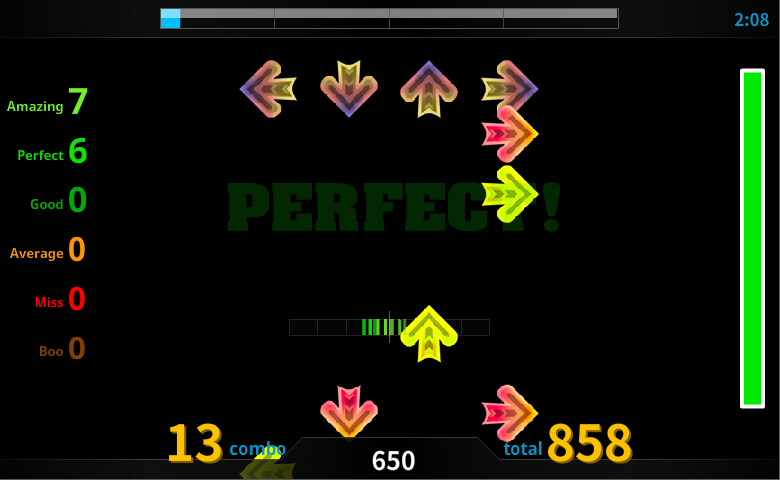
\includegraphics[width=15cm]{reports/figures/images/gameplay.png}
\captionof{figure}{Screenshot of FFR's Gameplay View (upscroll view)}
\label{fig:gameplay}
\end{center}

The implementation of the life bar introduces two potential scenarios that require further investigation: situations in which the difficulty of executing these playing objectives remains independent of the life bar, and cases in which it becomes dependent on it.

\vspace{2mm}

\textit{Case One:} \textbf{Life Bar Independent}

\vspace{2mm}

\textit{Case Two:} \textbf{Life Bar Dependent}

\vspace{2mm}
In this case, the life bar is the primary factor responsible for the difficulty of accomplishing these scoring-based objectives. Particularly, because Boos are generated at a higher rate compared to other judgements, excessive generation of Boos runs the risk of causing the player to fail the level. Conversely, getting too many hits (e.g. Perfects, Goods, and Averages) can result in missed chances to acquire sufficient Misses and Boos needed to attain the desired score.

\vspace{2mm}

The life bar can be redefined as a one-dimensional random walk with a reflective barrier at position $20$ and an absorbing barrier at position $0$. All possible states of the life bar can be defined by the particle's position. Starting from position $10$, positive movements of the particle represent successful hits, regardless of the judgement received, while negative movements represent either hitting a non-existent note (Boo) or missing an existing note (Miss). Using the random walk analogy, we begin by proposing the following conjecture:

\begin{conjecture}
Let $g(n)$ represent the number of ways a player can fail passing a stepfile with at most $n$ actions, where actions are either categorized as ``hits" (i.e. Perfects, Goods, Averages) or ``no-hits" (i.e. Miss, Boos). Then,

$$g(n) \sim \binom{n}{\lfloor\frac{n-10}{2}\rfloor}$$
\end{conjecture}

Note that Misses and Boos are treated as independent ``no-hits" while Perfects, Goods, and Averages are interpreted as one ``hit". 

\vspace{2mm}

    Define $f(n, k)$ to represent the number of possible combinations of $n$ actions that result in a total of $k$ health during gameplay. When no actions have been executed ($n = 0$), there exists only one possible scenario in which a total of $k = 10$ health is obtained, while all other possible outcomes for $k$ will be $0$, considering that every player begins with $10$ health. Therefore, 
    $$f(0, k) = \begin{cases} 
          1 & k = 10 \\
          0 & \text{otherwise}
       \end{cases}$$
    
    In the case where $k > 0$ and the barriers are not present, achieving a health level of $k$ after $n$ actions would require performing the correct action at either $k-1$ or $k+1$ health after $n-1$ actions. However, at the reflecting barrier, where $k+1$ health is unattainable, reaching $k$ health would necessitate arriving at $k$ health after $n-1$ actions. As such, the recursive formulation for $f(n, k)$ can be expressed as:
    $$f(n, k) = \begin{cases} 
          f(n-1, k - 1) + f(n-1, k) & k = 20 \\
          f(n-1, k - 1) + f(n-1, k+1) & 0 \leq k < 20 \\
          0 & \text{otherwise}
       \end{cases}$$

    Define $g(n)$ as follows:

    $$g(n) = \sum_{m=0}^n f(m, 0).$$

    When we expand the recursion and compute $g(n)$, without sufficient proof, we claim that

    $$g(n) = \binom{n}{\lfloor\frac{n-10}{2}\rfloor} + O(n^2).$$


\subsection{Machine Learning Problem Formulation}

We will begin this section by introducing some definitions and proposing a theorem:

\begin{itemize}
    \item \textit{Objective stepfile features} refer to characteristics of a stepfile that contain rigid requirements independent of the player's skill level. These may include precise timing requirements for all arrows and the duration of the stepfile. Note that meta stepfile features are not considered objective, as the established definition to differentiate patterns from one another cannot be codified deterministically. 
    \item \textit{Subjective stepfile features} are defined as elements that are primarily centered on the execution of the stepfile and are subject to the player's individual skill level. These features may include factors related to a player's ability to execute the steps accurately, as well as their access to high-quality equipment. For instance, a player with greater stamina is likely to excel at longer stepfiles and may tend to underestimate its level of challenge as a result. 
\end{itemize}

\begin{theorem}
Given a stepfile, the true difficulty rating can be estimated with a machine learning model using the objective stepfile features and the upper echelons of player telemetry.
\end{theorem}

\begin{proof}
Let Players $A_1, A_2, \cdots, A_n$ represent $n$ players to provide feedback on the stepfile difficulty of a given stepfile. Each time Player $A_i$ for all $1 \leq i \leq n$ makes an assessment on the difficulty of the stepfile, they rely on both unique characteristics of the stepfile and their individual skill sets
to justify this claim. Under the assumption that stepfile difficulty is additive, this can captured in the following equation:

$$\text{Diff}_{\text{obs}}^{(A_i)} = \text{Diff}_{\text{obj}}^{(A_i)} + \text{Diff}_{\text{sub}}^{(A_i)}.$$

Because each player $A_1, A_2, \cdots, A_n$ are exposed to the same step layout in a given stepfile, their unbiased assessments of difficulty are mutually shared. This can be mathematically expressed as follows:

$$\text{Diff}_{\text{obj}} \coloneq \text{Diff}_{\text{obj}}^{(A_1)} = \text{Diff}_{\text{obj}}^{(A_2)} = \cdots = \text{Diff}_{\text{obj}}^{(A_n)}.$$

Define $A = (A_1, \cdots, A_n)$ to represent a community of $n$ players. When we aggregate all $n$ player's difficulty assessments, we can determine the observed difficulty rating of a stepfile subject to community bias:

$$\text{Diff}_{\text{obs}}^{(A)} = \text{Diff}_{\text{obj}} + \text{Diff}_{\text{sub}}^{(A)}.$$

In theory, by obtaining feedback from the entire population regarding the difficulty of a stepfile, with an unlimited sample (i.e. $n \rightarrow \infty$), it may be possible to establish an accurate measurement of difficulty that considers human limitations and reduces the influence of player subjectivity. Therefore, for some constant unknown value $\text{Diff}_{\text{human}}$, we have the following:

$$\lim_{n \rightarrow \infty} \text{Diff}_{\text{obs}}^{(A)} = \text{Diff}_{\text{true}}\mspace{50mu} \text{and} \mspace{50mu} \lim_{n \rightarrow \infty} \text{Diff}_{\text{sub}}^{(A)} = \text{Diff}_{\text{human}}.$$

Using the above asymptotics, we can conclude that
$$\text{Diff}_{\text{true}} = \text{Diff}_{\text{obj}} + \text{Diff}_{\text{human}}.$$
\end{proof}

Note that the current difficulty ratings in game are notated as $\text{Diff}_{\text{obs}}^{(A)}$ in the previous proof. Based on this, we propose the following corollary:

\begin{corollary}
The deviation between $\text{Diff}_{\text{true}}$ and $\text{Diff}_{\text{obs}}^{(A)}$ is largely dependent on subjective features of the stepfile defined by the vocal community. In other words,

$$|\text{Diff}_{\text{obs}}^{(A)} - \text{Diff}_{\text{true}}| = |\text{Diff}_{\text{sub}}^{(A)} - \text{Diff}_{\text{human}}|$$
\end{corollary}

In order to ensure the credibility of the given target values, it is crucial to minimize the deviation between $\text{Diff}_{\text{obs}}^{(A)}$ and $\text{Diff}_{\text{true}}$. From the above corollary, this can be accomplished by utilizing community feedback to estimate $\text{Diff}_{\text{human}}$, the role which difficulty consultants play when receiving new opinions from community members. This requires us to gather more feedback from the community, which is highly susceptible to self-selection bias and group attribution error.

\vspace{2mm}

Instead of attempting to correct data labeling errors, we will use the ratings as targets in our supervised learning problem to estimate the true difficulty $\text{Diff}_{\text{true}}$ by maximizing the explained variation of the objective stepfile features. Doing so enables us to rely less on our inability to control identified biases in our analysis, while creating future opportunities to improve the definition of true difficulty through through continued research on player telemetry and improved feature engineering from available stepfile data.
\vspace{2mm}

Let's assume that there is some relationship between $Y \coloneq  \text{Diff}_{\text{true}}$ and features $X_{\text{obj}} = (X_{\text{obj}}^1, \cdots, X_{\text{obj}}^n)$ which can be written in the very general form:

$$Y = f(X_{\text{obj}}) + \epsilon$$

where $f$ is some fixed and unknown function of $X_{\text{obj}}^1, \cdots, X_{\text{obj}}^n$ and $\epsilon$ is a random error term, independent of $X_{\text{obj}}$ and has mean zero. Given our previously stated goal, it is important to note that the error term is specifically formulated to account for the explained variance of stepfile difficulty that can be attributed to inherent human limitations.

\vspace{2mm}

Let $\hat{f}$ be an estimate of $f$ that yields prediction $\hat{Y} = \hat{f}(X_{\text{obj}})$. Assume for a moment that both $\hat{f}$ and $X_{\text{obj}}$ are fixed. Then,
\begin{align*}
    E(Y - \hat{Y})^2 & = E(f(X_{\text{obj}}) + \epsilon - \hat{f}(X_{\text{obj}}))^2 \\
    & = [f(X_{\text{obj}}) - \hat{f}(X_{\text{obj}})]^2 + \text{Var}(\epsilon)
\end{align*}

The main objective of our research is to accurately calculate the function $f$, while also minimizing the reducible error $[f(X_{\text{obj}}) - \hat{f}(X_{\text{obj}})]^2$. It is important to acknowledge that the features selected in this study will comply with inferential properties related to stepfile difficulty, as further explained in a subsequent section.

\vspace{2mm}






\textbf{Plan:}
\begin{itemize}
	      	      
	      \item{Introduce Contested Difficulty Sheet and define train-test split using KDE estimations of proposed difficulties}
	      	      
	      \item{Introduce objective features VerticalDensity and HorizontalDensity using pen-tapping as an example. Also mention chart augmentation considerations:}
	      \begin{itemize}
	      	\item Mirror: Indirectly accounted in VerticalDensity's definition
	      	\item Offset: Indirectly accounted in preprocessing of FFR's API response.
	      	\item Colors: Categorized under "processing difficulty"; users can alter this.
	      	\item Scroll Speed Mod: Categorized under "processing difficulty"; users can alter this.
	      \end{itemize}
	      	      
	\item Dissociate local features from global features. Song length is a global feature, subsequence extraction is a local feature. Mention how ensembling works with the consideration of "difficulty spikes" in many charts.
	      	      
	\item Introduce model architecture and implementation. Consider regressing over the target variable transformations of difficulty due to domain knowledge of difficulty.
	      	      
	\item Run experiments with proposed model, share results, and identify method to measure the quality of the predictions.
	      	      
	\item Extend proposed model to account for uprated and downrated stepfiles, run experiments and compare model performance with already tracked uprated scores.
	      	          
\end{itemize}

\vspace{2mm}


% In addition to issues mentioned earlier in this report, the evolution of FFR's stepfile difficulty measurement demonstrates the varying perspectives on what constitutes a challenging stepfile. A notable factor contributing to this lack of a consensus is the absence of standardized criteria for determining difficulty. This section aims to establish such standards in order to establish a more reliable and trusted model for evaluating stepfile difficulty, by examining the Contested Difficulties spreadsheet and identifying the difficulty values that hold the most consensus within the FFR community.

\subsection{Contested Difficulty Spreadsheet Analysis}

The Contested Difficulty Spreadsheet, managed by \texttt{Zlyice}, is a collaborative Google Sheets document utilized for tracking proposed changes to stepfile difficulty measurements based on input from users. It is presumed that the individual suggesting a difficulty measurement possesses a degree of knowledge regarding the factors that warrant such a rating for the stepfile. While it must be acknowledged that all proposed measurements are inherently vulnerable to volunteer bias, the process of crowd-sourcing these partial inputs serves to reduce the impact of individual bias on any given stepfile. This approach aims to align the definition of difficulty with the perspectives of the vocal minority within the wider community.

\vspace{2mm}


In order to align our model scoring with the prevailing consensus on the quantification of stepfile difficulty within the community, we conduct a thorough analysis of the proposed difficulty levels over the period spanning from 2022 to the present date. This analysis serves as the basis for our development of a train-test split strategy, in which the distribution of proposed difficulties is utilized to allocate our data into appropriately representative training, validation, and test sets.